\section{Trigger Labeling}\label{trigger}
Trigger labeling, also called event detection, aims to discover event triggers and assign them a predefined event type. We jointly learn trigger identification and type classification by one network to reduce the error propagation problem in a pipeline model. Before we present our solution, we first discuss the language specific issues in Chinese trigger labeling.

\subsection{Language Specific Issues}
We summarize the inconsistency problems between words and triggers as the following two types.

\begin{enumerate}
	\item Cross-word triggers: While many events anchor on a single word, multiple words could reasonably be called a trigger. In S4, the \emph{arrest\_jail} event should be triggered by neither ``落入'' nor ``法网'', but ``落入法网'' (arrested).
	\item Inside-word triggers: Almost all Chinese characters have their own meanings, and some of which can be triggers themselves. There may be greater than one trigger in a word like ``击毙'' (shoot and kill). Continuous characters of a word can also form a trigger such as ``凶杀'' (murder) in ``凶杀案'' (murder case).
\end{enumerate}

Table~\ref{tab:one} summarizes the number of problematic triggers we found in ACE 2005 Chinese corpus using different Chinese word segmentation tools. Even the minimum inconsistency rate is as high as 14\%.

\begin{savenotes}
\begin{table}
\centering
\tbl{Numbers of triggers inconsistent with the words.\label{tab:one}}{
\begin{tabular}{lccc}
\toprule
\textbf{NLP Tool} & \textbf{Cross-word Trigger} & \textbf{Inside-word Trigger} & \textbf{Total} \\ \midrule
\rowcolor{Gray} Stanford NLP\footnote{\texttt{http://nlp.stanford.edu/software/segmenter.shtml}} & 14.6\% & 5.0\% & 19.6\% \\
Jieba\footnote{\texttt{https://github.com/fxsjy/jieba}} & 16.6\% & 2.6\% & 19.2\% \\
\rowcolor{Gray}  NLPIR\footnote{\texttt{https://github.com/NLPIR-team/NLPIR}} & 8.9\% & 5.2\% & 14.1\% \\
\bottomrule
\end{tabular}}
\end{table}
\end{savenotes}

To address the language specific issues, we treat event detection as a sequence labeling task. Formally, we use $\bm{w}=\{w_1, w_2, \ldots, w_n\}$ to represent an input sentence of length $n$, where $w_i$ is the $i$-th word. And $\bm{y}=\{y_1, y_2, \ldots, y_n\}$ represents a generic sequence of labels for $\bm{w}$. Each word is tagged in the \texttt{BIO} scheme, where each token is labeled as \texttt{B-type} if it is the beginning of an event trigger with event type \texttt{type}, or \texttt{I-type} if it is inside a trigger, or \texttt{O} otherwise. Our first labeling model is a word-based bidirectional LSTM network (BiLSTM) with a CNN layer as shown in Figure~\ref{fig:1}.

\subsection{Word-based Convolution BiLSTM Model \label{wcblstm}}
In this section, we introduce the components (layers) in our Convolution BiLSTM (C-BiLSTM) network one-by-one from bottom to top.
\begin{figure}
\centering
\subfigure[Convolution BiLSTM network]{\label{fig:a}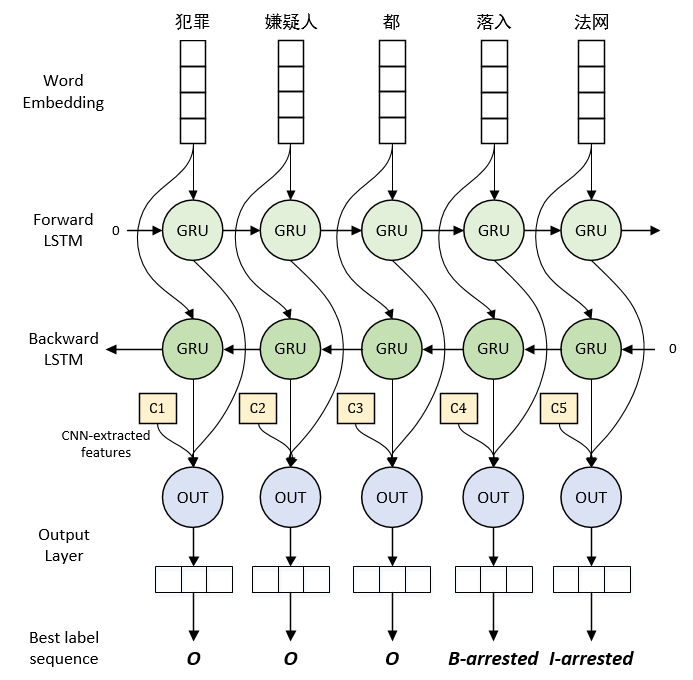
\includegraphics[width=0.62\textwidth]{RNN1.png}}
\subfigure[Details of CNN in (a)]{\label{fig:b}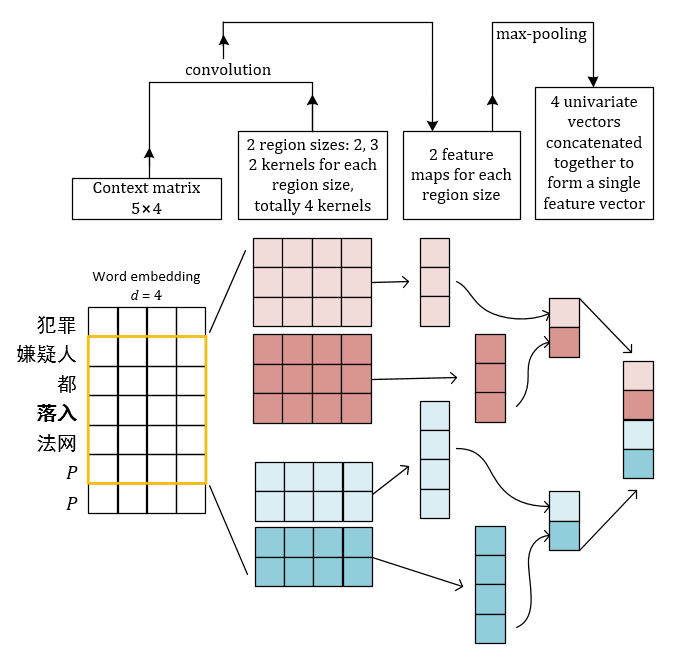
\includegraphics[width=0.62\textwidth]{CNN1.png}}

\caption{The main architecture of our word-based convolution bidirectional LSTM model. The local contextual feature $c_{i}$ (yellow rectangle) in (a) for each word $w_i$ is computed by the CNN as (b) illustrated. Our CNN layer learns a representation of local context information about the center word ``落入''. Here the context size is 5 (2 words to the left and to the right of a center word), and we depict two kernel region sizes: 2 and 3, each of which has 2 kernels. The symbol \emph{P} in sentence of (b) represents a padding word.\label{fig:1}}

\end{figure}

\paragraph{LSTM Network}
Recurrent neural networks (RNNs) maintain a memory based on historical contextual information, which makes them a natural choice for processing sequential data. Unfortunately, it is difficult for standard RNNs to capture long range dependencies due to vanishing/exploding gradients \cite{bengio1994learning}. Long Short-Term Memory Network \cite{hochreiter1997long} is explicitly designed to solve the long-term dependency problem through purpose-built memory cells. They consist of several multiplicative gates that control the proportion of information to forget and to store in the cell states. In this paper, we apply a variation of LSTM units, Gated Recurrent Unit (GRU) \cite{cho2014learning}, which is found to be superior to LSTM on a suit of tasks by Chung et al. \shortcite{chung2014empirical}. The GRU is implemented as the following formulas:
\begin{align*}
	\text{r}_t &= \sigma(\text{W}_{xr}\text{x}_t + \text{W}_{hr}\text{h}_{t-1} + \text{b}_r) \\
	\text{z}_t &= \sigma(\text{W}_{xz}\text{x}_t + \text{W}_{hz}\text{h}_{t-1} + \text{b}_z) \\
	\tilde{\text{h}}_t &= \tanh(\text{W}_{xh}\text{x}_t + \text{W}_{hh}(\text{r}_t \odot \text{h}_{t-1}) + \text{b}_h) \\
	\text{h}_t &= \text{z}_t \odot \text{h}_{t-1} + (1 - \text{z}_t) \odot \tilde{\text{h}}_t
\end{align*}

In these formulas, the $\text{W}_*$ variables are the weight matrices and the $\text{b}_*$ variables  are the biases. $\sigma(\cdot)$ is the element-wise sigmoid function and $\odot$ is the element-wise product.

Formally, we use $\text{x}_t$ to represent the feature vector (e.g. word embedding) corresponding to the $t$-th word $w_t$. At each time step $t$, a GRU takes $\text{x}_t$ as input and computes the hidden state (also called output vector) $\text{h}_t$ by reset gate and update gate. The reset gate $\text{r}_t$ controls how much and what information from the previous hidden state should be reset, and the update gate $\text{z}_t$ determines how much the unit updates its previous hidden state.

\paragraph{BiLSTM Network}
In the event extraction task, if we can access to both past and future contexts for a candidate trigger, we can explore richer sentence-level information and make better prediction. This can be done by bidirectional LSTM networks \cite{graves2005framewise,graves2013speech}. Figure 1(a) shows the layers of a BiLSTM trigger identification model.

At time $t$, a forward LSTM network computes the hidden state $\overrightarrow{\text{h}_t}$ of the past (left) context of the sentence at word $w_t$, while a backward LSTM network reads the same sentence in reverse and outputs $\overleftarrow{\text{h}_t}$ given the future (right) context. We concatenate these two vectors to form the output vector of a BiLSTM network, i.e. $\text{B}_t = [\overrightarrow{\text{h}_t}; \overleftarrow{\text{h}_t}]$.

\paragraph{CNN Layer}
Convolutional neural networks (CNNs) are originally applied to computer vision to capture salient local features \cite{lecun1998gradient}. Previous studies on event extraction \cite{nguyen2015event,chen2015event,feng2016language} have gradually shown that CNN architectures are effective to capture semantic features similar to n-grams, but represent them in a more compact way. We employ a convolutional neural network as illustrated in Figure 1(b) to extract local contextual information for each word in a sentence.
Specifically, for every word in the sentence, we want to extract local contextual information to help predict whether the current word is an event trigger. The current word $w_i$ along with its context constitutes the input of CNN. Let $w_{i:i+j}$ be the window of words from $w_i$ to $w_{i+j}$, and $2k+1$ be the fixed context size. So the context window $c_i$ (padded when necessary) where the current word $w_i$ is in the middle can be written as
\begin{equation}
	c_i = w_{i-k:i+k} = [w_{i-k}, \ldots, w_{i}, \ldots, w_{i+k}].
\end{equation}
Before being fed into a convolution layer, each word $w_i$ is transformed into a d-dimensional word vector $\text{x}_i$ by looking up the embedding table. As a result, the original context $c_i$ is transformed into a matrix $\bm{c}_i = [\text{x}_{i-k}, \ldots, \text{x}_i, \ldots, \text{x}_{x+k}]$ of size $(2k+1) \times d$. The matrices $\bm{c}_1$, \ldots, $\bm{c}_n$ are then passed through a convolution layer and a max pooling layer.
In the convolution layer, we utilize a set of kernels $\{\text{w}_1, \text{w}_2, \ldots, \text{w}_m\}$ with various widths to extract semantic features like n-grams of different granularities. For every context matrix $\bm{c}_i$, a kernel $\text{w}_j$ of width $l$ is applied to all possible windows of $l$ words within the context (i.e., $w_{i-k:i-k+l-1}$, \ldots, $w_{i+k-l+1:i+k}$). And $\text{w}_j$ can be essentially seen as a weight matrix of size $l \times d$. For example, the convolution operation involves kernel $\text{w}_j$ over the window $w_{t:t+l-1}$ can be express as:
\begin{equation} s_{jt}=f(\text{w}_j \cdot \text{x}_{t:t+l-1} + b_j), 1 \leq j \leq m, i-k \leq t \leq i+k-l+1 \end{equation}
where $b$ is a bias term and $f$ is a non-linear function such as hyperbolic tangent. The convolution result is a feature map $\text{s}_j \in \mathbb{R}^{2k-l+2}$.
We then perform a max-over-time pooling operation \cite{collobert2011natural} over each feature map,
\begin{equation}
\tilde{s}_j=\max\{\text{s}_j\}=\max\{s_{j1}, s_{j2}, \ldots, s_{jm}\}	
\end{equation}
so that only the largest number is recorded. One property of pooling is that it produces a fixed size output vector, which enables us to apply variable kernel sizes. And by performing the max operation, we are keeping the most salient information. Finally, we take the fixed length output vector $\text{C}=[\tilde{s}_1, \tilde{s}_2, \ldots, \tilde{s}_m]$ as a representation of local contextual information about the current word.

In our implementation, the context window size is 7 (3 words to the left and to the right of a center word), and kernel sizes from 2 to 7 to encode the semantics of n-grams with various granularities. Each kernel generates 32 feature maps.

\paragraph{Output Layer\label{output}}
For each word $w_i$ in the sentence, we concatenate the bidirectional sentence-level features $\text{B}_i$ learned by BiLSTM, and the contextual semantic features $\text{C}_i$ extracted by CNN, into a single vector $\text{F}_i=[\text{B}_i;\text{C}_i]$. To compute the confidence of each label, the final feature vector $\text{F}_i \in \mathbb{R}^{2d_{gru}+d_{cnn}}$, where $d_{gru}$ is the dimension of the GRU unit and $d_{cnn}$ is the number of feature maps in CNN layer, is fed into a fully connected linear layer.
\begin{equation}
	 \text{O}_i = \text{W}_s\text{F}_i+\text{b}_s
\end{equation}

where $\text{W}_s \in \mathbb{R}^{n_{e} \times (2d_{gru} + d_{cnn})}$ is the transformation matrix and $\text{O}_i=[O_{i,1}, \ldots, O_{i,{n_e}}]$ is the final output vector, $n_{e}$ is the number of distinct labels, and the $e$-th element $O_{i, e}$ indicates the score for label $e$.

Then $\text{O}_i \in \mathbb{R}^{n_e}$ is fed into a softmax layer to estimate a probability distribution over all possible labels. In the end, we choose the label that obtains maximum probability as the prediction for $y_i$.
\begin{equation}
	P(e \mid \text{O}_i) = \frac{\exp{(O_{i,e})}}{\sum\nolimits_{j=1}^{n_e}\exp{(O_{i,j})}}
\end{equation}
\begin{equation}
  	y_i = \argmax\limits_{e}{P(e \mid \text{O}_i)}
\end{equation}

\paragraph{Errata Table}
However, this word-base model still suffer from  the inconsistency problem caused by inside-word triggers. Inspired by \citeN{chen2009language}, we construct a global errata table to record some frequent appearances of tokens and triggers in the training set. In our experiments, if 80\% occurrences of a token inside a word should be labeled as triggers with the same event type, we then add this ``word$-$token$-$type'' triple into the table. During testing, if a word has an entry in the errata table, we regard its token as a trigger with the event type according to the corresponding triple directly. For example, if ``击毙$-$击$-$\emph{Attack}'' and ``击毙$-$毙$-$\emph{Die}'' are two triples in the errata table, word-based C-BiLSTM model can identify all inside-word triggers in S6 correctly.

\subsection{Character-based Convolution BiLSTM Model \label{ccblstm}}
\begin{figure}
\centering
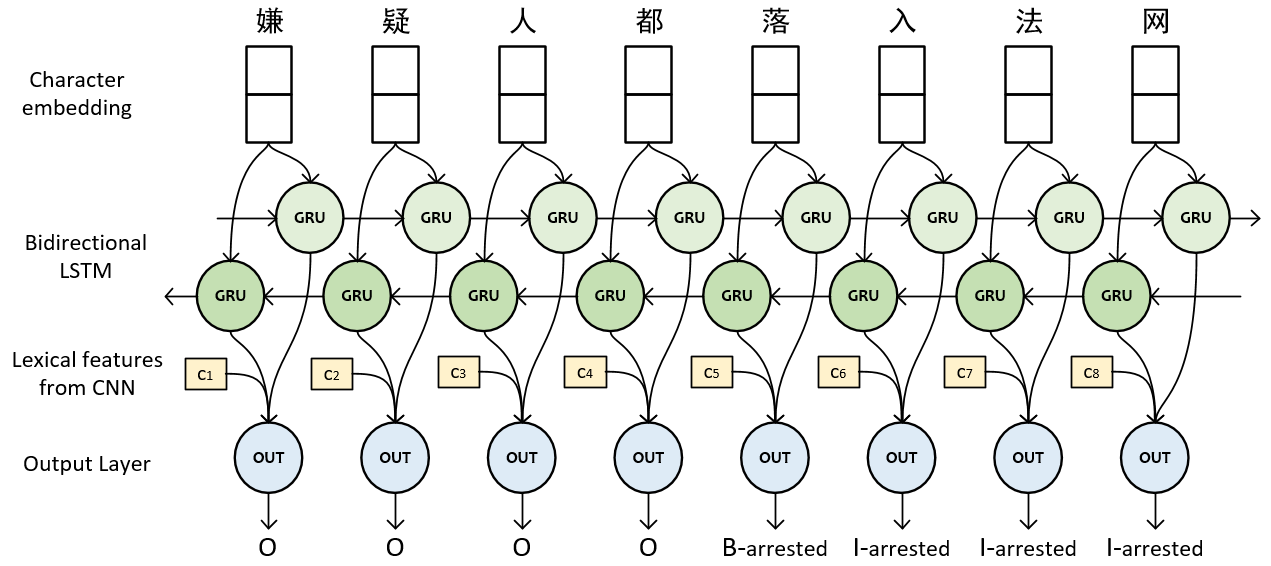
\includegraphics[width=.9\textwidth]{RNN2.png}
\caption{Character-based Convolution BiLSTM network.}
\label{figure2}
\end{figure}

Despite of the effectiveness of errata table, word-based method is not a perfect solution to language specific issues, because it only recognizes triggers in a word level or frequent inside-word triggers appearing in training data. When it comes to an unknown inside-word trigger which never occurs during training, there is no way for an errata table to label it correctly.

Ideally, character-based methods may solve both inconsistency problems, which use the same \texttt{\{BIO\}-type} tagging scheme as word-based model, however, to label each character rather than each word. For better understanding, resulting sequences of example sentences S4 and S5 labeled by two models are listed in Table~\ref{six}.

As shown in Figure~\ref{figure2}, character-based C-BiLSTM has a similar network architecture as word-based C-BiLSTM. The main difference is that character-based model tags a sentence character by character, while word-based model tags a sentence word by word. They also differ in their input layers: character-based C-BiLSTM uses character embeddings as input feature vectors, while word-based C-BiLSTM utilizes word embeddings.

\begin{table}
\newcommand{\tabincell}[2]{\begin{tabular}{@{}#1@{}}#2\end{tabular}}
\tbl{Difference of output sequences between character-based method and word-based method \label{six}}{
\begin{tabular}{rl} \toprule
Sentence: & \tabincell{l}{
犯罪 \hspace{0.1cm}嫌疑人 \hspace{0.2cm}都 \hspace{0.2cm}\textbf{落入 法网}。 \\
The suspects were \textbf{arrested}.} \\
\midrule
C-BiLSTM$_{word}$: & \texttt{ O \hspace{0.45cm}O \hspace{0.3cm}O \hspace{0.75cm}B-arrested \hspace{1.5cm}I-arrested} \\
C-BiLSTM$_{char}$: & \texttt{O O O O O O B-arrested I-arrested I-arrested I-arrested} \\
\bottomrule

Sentence: & \tabincell{l}{ \hspace{0.15cm}警察 \hspace{0.85cm}\textbf{击毙} 了 \hspace{0.1cm}一名 \hspace{0.15cm}歹徒。\\
Polices \textbf{shoot} and \textbf{kill} a criminal.} \\
\midrule
C-BiLSTM$_{word}$: & Can not label this sentence correctly. \\
C-BiLSTM$_{char}$: & \texttt{O O B-attack B-die O O O O O} \\
\bottomrule
\end{tabular}}
\end{table}

\subsection{Character-based Convolution BiLSTM-CRF Model}
As mentioned in Section ~\ref{output}, regarding the final feature vector $\text{F}$ as an input to a softmax classifier is a straightforward but effective way to make independent labeling decisions. However, the independent classification decisions are limited when there are strong dependencies between tags in a sentence. For example, in trigger labeling, \texttt{B-attack} is more likely to be followed by \texttt{B-die}, while \texttt{I-die} cannot follow \texttt{B-attack}. \textbf{Output layers in C-BiLSTM models cannot exploit this sentence level labeling information.}

Therefore, we propose a character-based convolution BiLSTM-CRF model (C-BiLSTM-CRF) that considers the correlations between labels in neighborhoods and jointly decodes the best sequence of labels via a CRF layer. This kind of CRF architecture is similar to the ones presented in other sequence labeling tasks, such as chunking and NER \cite{collobert2011natural,huang2015bidirectional,lample2016neural}.

Given an input sentence
\begin{displaymath}
	\bm{X} = (\text{x}_1, \text{x}_2, \ldots, \text{x}_n),
\end{displaymath}
we consider $\bm{P}$ to be a matrix of confidence scores output by C-BiLSTM network.
\begin{equation}
	\bm{P} = [\text{O}_1, \text{O}_2, \ldots, \text{O}_n]
\end{equation}
$\bm{P}$ is of size $n \times e$, where $e$ is the number of distinct tags, and $P_{i,j}$ correspond to the confidence of the $j$-th tag for the $i$-th word in a sentence.

We introduce a state transition matrix $\bm{A}$ in CRF layer such that $A_{i,j}$ represents the score of a transition from label $i$ to label $j$. We take into account neural network outputs and transition scores, and score a sentence $\bm{X}$ along with a path of labels $\bm{y}=\{y_1, y_2, \ldots, y_n\}$ to be
\begin{equation}
	score(\bm{X}, \bm{y}) = \sum\limits_{i=0}^nA_{y_i, y_{i+1}} + \sum\limits_{i=1}^nP_{i, y_i},
\end{equation}
where $y_0$ and $y_{n+1}$ are the special labels, \texttt{start} and \texttt{end}, that we add to the set of possible labels. $\bm{A}$ is therefore a square matrix of size $(e+2) \times (e+2)$.

We normalize this score over all possible label sequences $\tilde{\bm{y}}$ using a softmax, and we interpreted the resulting ratio as a conditional label sequence probability:
\begin{equation}
	p(\bm{y}|\bm{X})=\frac{\exp({score(\bm{X}, \bm{y})})}{\sum\nolimits_{\tilde{\bm{y}} \in \bm{\mathcal{Y}}} \exp({score(\bm{X}, \tilde{\bm{y}})})}.
\end{equation}
where $\bm{\mathcal{Y}}$ represents all possible label sequences, including those invalid \texttt{BIO} scheme.

During training, for a dataset $\mathcal{T}$, we want to maximize the following logarithm of likelihood with respect to parameters $\tilde{\theta}$, which contains all neural network parameter $\theta$ and transition score matrix $\bm{A}$ in the CRF layer.
\begin{align}
L(\tilde{\theta}) &= \sum\nolimits_{(\bm{X}, \bm{y}) \in \mathcal{T}}{\log{(p(\bm{y}|\bm{X}))}} \\
\log{(p(\bm{y}|\bm{X}))} &= score(\bm{X}, \bm{y}) - \log{(\sum\nolimits_{\tilde{\bm{y}} \in \bm{\mathcal{Y}}} \exp({score(\bm{X}, \tilde{\bm{y}})}))} \notag	 \\
\label{e10}
&= score(\bm{X}, \bm{y}) - \logadd\limits_{\tilde{\bm{y}} \in \bm{\mathcal{Y}}}score(\bm{X}, \bm{\tilde{y}})
\end{align}
Although the number of terms in the $\logadd$ operation in Equation (\ref{e10}) is equal to the size of $\bm{\mathcal{Y}}$, which grows exponentially with the length of the sentence, we can compute it in linear time, proved by Collobert et al.\shortcite{collobert2011natural}.

At test time, given a sentence $\bm{X}$ to label, we have to find the best label sequence with the maximum score given by:
\begin{equation}
	\bm{y}^* = \argmax\limits_{\tilde{\bm{y}} \in \bm{\mathcal{Y}}}score(\bm{X}, \bm{\tilde{y}})
\end{equation}
Naturally, this inference can be solved efficiently by adopting the Viterbi algorithm \cite{rabiner1989tutorial}.
